\chapter{Наночастицы в опытах по разрушению скальных пород взрывом} \label{chapt3}

В настоящей работе приведены результаты дальнейших экспериментальных исследований (продолжение работы [1, 11]) наномасштабных частиц, образованных при массовых взрывах.  Выявление закономерностей новообразования частиц в зависимости от параметров взрывов (вида ВВ, удельного расхода и т.д.), а также от типа горной породы и ее физико–механических свойств, подразумевает в итоге возможность управления процессом формирования наномасштабных частиц при взрывах. Образование частиц наномасштабного размера важно для решения некоторых экологических проблем, связанных с загрязнением окружающей среды.
Продолжением ранее опубликованных исследований по формированию нано- и микромасштабных частиц при разрушении скальных пород взрывом [1, 11] послужило рассмотрение характеристик частиц малых размеров, образованных в результате последовательных пяти взрывов. Последовательные взрывы изменяет в образцах относительные соотношения количества частиц, образованных различными механизмами, что необходимо для более детального изучения этих механизмов и их вкладов в образование нано- и микромасштабных частиц.

Набор образцов грунта для проведения исследования размерно–массовых соотношений в диапазоне от нанометров до миллиметров был получен в результате серии, состоящей из пяти взрывов, в гранитном массиве Фенноскандии около г. Выборга. Характерной особенностью гранитов района является однородность их текстуры — порода массива содержит порфировидные вкрапления калиевого полевого шпата, которые имеют размеры от 3–5 см до 0.5–2 см и составляют от 36 до 43\% массы породы. Пространство между вкраплениями заполнено крупно– и мелкозернистой массой, состоящей из кварца (23–33\%), плагиоклазов (18 − 24\%), биотита (до 8\%) и роговой обманки (до 7\%). Скорость распространения продольных волн в поверхностной части массива находится в пределах   м/с, плотность гранита   кг/м3. Источниками взрыва служили шашки прессованного тротила весом 200 г. Плотность тротила составляет 1.5 г/см\textsuperscript{3}, теплота взрыва — 4120 кДж/кг, скорость детонации 6000 м/с, давление в волне детонации МПа[1]. 
Последовательность получения образцов была следующей: первый образец был получен из воронки, образованной после взрыва заряда на гладкой гранитной площадке, второй — после взрыва в образованной воронке и т.д. Масса образцов грунта – от 5 до 25 гр. Все образцы были последовательно просеяны через сита размером 2,5; 1,6; 1; 0,63; 0,4; 0,315; 0,2; 0,16 и 0,04 мм. Все фракции взвешивались и затем строились предварительные распределения количества частиц по размерам для диапазона 0,040—2,5 мм в координатах Розина–Раммлера. Фракция меньшая 40 мкм была разделена на порции пригодные для анализа на растровом  электронном микроскопе. Анализ частиц из образцов грунта размером менее 40 мкм проводился на растровом электронном микроскопе JEOL 6460 LV.

Для удобства получения информации о размерах частиц на снимках, полученных с помощью электронного микроскопа, было реализовано программное обеспечение. При работе с ним по масштабной линейке определяется масштаб и площадь снимка. Затем пользователь, рисуя мышью прямоугольники, (см. рис.~\ref{img:3app}) выделяет частицы, размером приблизительно входящие в заданный заранее диапазон. Размер частицы вычисляется из размера диагонали прямоугольника, разделенного на (таким образом, образуя альтернативный средний квадрат). В дальнейшем проводится обобщение результата обработки снимка путем пересчета индивидуальных размеров в данные по количеству частиц на заданные заранее интервалы.
Для анализа и трактовки распределений частиц выполнялось сравнение распределений, полученных в опытах, с теоретическими распределениями Розина–Раммлера и Колмогорова. Для частиц с размером более 40 мкм отмечена хорошая согласованность с теоретическим распределением Розина–Раммлера, выведенного в предположении однократности дробления —  . Здесь $x$ – размер частицы; $V_{0}$ – объём исследованного вещества; $V(x)$ – общий объём частиц, размер которых больше $x$; $x_{0}$, $n$ – параметры распределения,   – среднемассовый размер частицы. От опыта к опыту, как и следовало ожидать, средний размер частиц и коэффициент распределения n уменьшаются, что свидетельствует о расширении грансостава в зависимости от числа предшествующих взрывов. 

\begin{figure} [h] 
  \center
  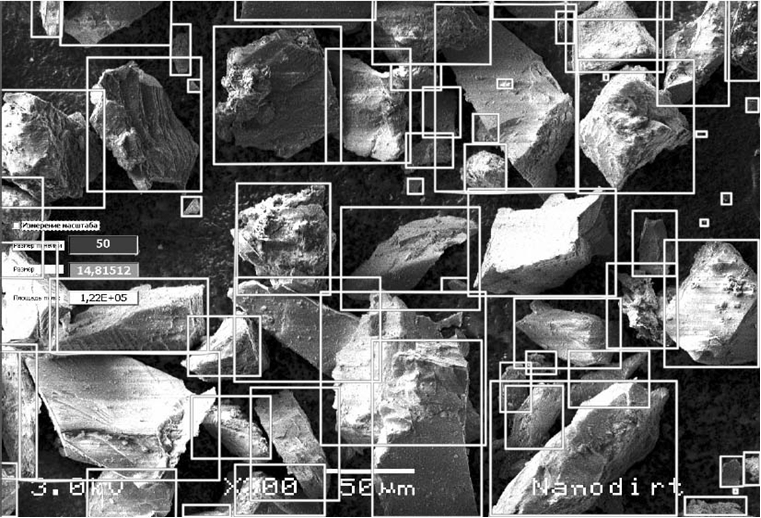
\includegraphics[width=160mm]{pic31}
  \caption{Рабочее окно, формируемое программным обеспечением, при обработке электронных изображений.} 
  \label{img:3app}  
\end{figure}

На рис.~\ref{img:3rr} в спрямляющих координатах, соответствующих распределению Розина–Раммлера, и во всем диапазоне размеров проведено сравнение распределения по размерам для частиц, образованных после третьего взрыва, (вычисленного на основе данных «сшивки» данных ситового анализа и электронной микроскопии) с линией тренда (в рамках распределения Розина–Раммлера по данным ситового анализа). Оказывается, что в области самых мелких частиц имеется достаточно сильное отклонение экспериментальной кривой от линии тренда, что свидетельствует о нехватке частиц (по сравнению с ситуацией, когда распределение точно соответствует распределению Розина–Раммлера).
Существенно лучшее соответствие получается в логнормальных координатах, соответствующих распределению Колмогорова (см. рис.~\ref{img:3k}), что свидетельствует о многократности дробления —   /12/. Здесь x – размер частицы; $Ф(t)$ – вероятность обнаружить частицу, размеры которой меньше $x$; ; $x_{0}$,   – параметры распределения,   – среднемассовый размер частицы. Наличие аномального количества какого–либо размера частиц, которое возникло бы из–за скопления, связанного с достижением предела прочности вещества породы, не отмечается.

\begin{figure} [h] 
  \center
  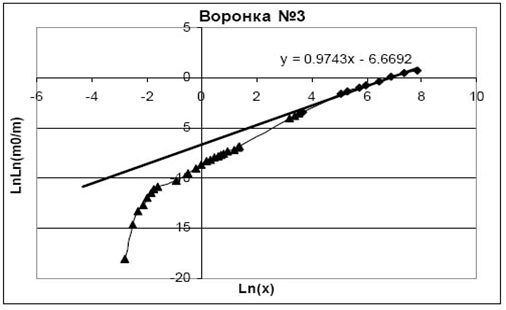
\includegraphics[width=110mm]{pic32}
  \caption{Кривая распределения частиц по размерам в спрямляющих координатах Розина–Раммлера для всего диапазона размеров частиц и линия тренда, полученная по данным ситового анализа.} 
  \label{img:3rr}  
\end{figure}

Итак, анализ нано- и микромасштабных частиц, образованных в результате одного или нескольких химических взрывов в гранитном массиве Фенноскандии около г. Выборга показал, что с ростом числа взрывов роль многократного дробления возрастает. После нескольких взрывов имеется лучшее соответствие полученного в экспериментах распределения частиц во всем диапазоне их размеров с распределением Колмогорова, чем с распределением Розина–Раммлера. При этом, в области достаточно больших размеров (больших 40 мкм) существенное место занимают частицы осколочной формы, подвергшиеся однократному дроблению. В пределах точности экспериментов в диапазоне исследуемых размеров, не проявляется усиление прочности материала, приводящее к возникновению предела прочности вещества породы, что обусловлено отсутствием участков на распределениях частиц по размерам, в которых наблюдалось бы аномально большое количество частиц тех или иных размеров.

\begin{figure} [h] 
  \center
  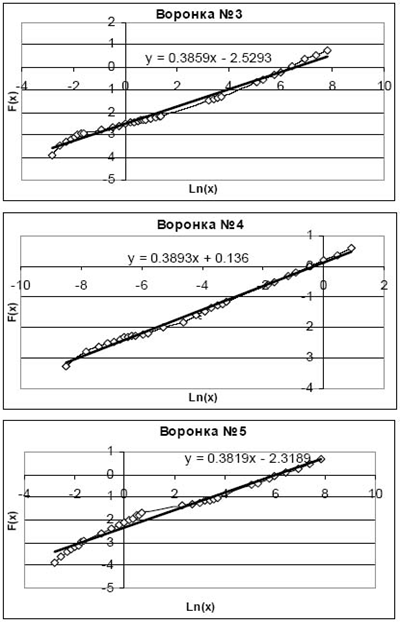
\includegraphics[width=110mm]{pic33}
  \caption{Сравнение распределений частиц, образованных после 3-го, 4-го и 5-го взрывов, в спрямляющих координатах, соответствующих распределению Колмогорова, с теоретическим распределением Колмогорова.} 
  \label{img:3k}  
\end{figure}

Таким образом, проведено исследование мелкодисперсных частиц нано- и микромасштабного размера, образующихся в результате разрушения горных пород как однократными, так и многократными взрывами химических ВВ. Выполнен статистический анализ мелкодисперсной фракции по размерам, и проведено сравнение с классическими распределениями Колмогорова и Розина–Раммлера. Доказана возможность образования наномасштабных частиц в результате разрушения породы взрывом с размерами, превосходящими 20 нм. Показано, что с ростом числа взрывов роль многократного дробления возрастает. Значительная часть наномасштабных частиц формируется вследствие дробления более крупных частиц, образованных при первом взрыве, во время последующих взрывов. В пределах точности экспериментов не выявлено усиления прочности материала при его дроблении до наномасштабных размеров.





\clearpage